\chapter{QUICK Box}
\label{chp:quickrollout} 

The main purpose of our study was to create an easy way to utilize the Mesh Potatoes in emergency situations and other situations where there are need for cheap and instant communication. Our main focus has been on providing Internet access to the mesh network formed by the \glspl{mp}, and on the aspect of quick roll-out of the network. The Internet may be a vital mean of communication in emergency situations, or just convenient in other situations. The process of setting up a mesh network providing Internet access should be done quickly, since time is a crucial factor to consider in emergency situations. In this chapter we will describe parts of the set-up techniques for the Mesh Potatoes. Further on we will present our \gls{quick} Box, which is a box including an \gls{mp}, a solar panel, a battery, a charge regulator, manuals for connecting the \gls{mp} to different uplinks, a manual describing how to get started with the box, necessary cables, a USB-stick containing script and a CD with Linux Ubuntu. A box ready to go in any situation. We will describe how we made this box, and similar work that has been conducted previously on this area. At last we will describe some situations where there is a need for a mobile communications system.

A big part of our work has been gathering of information, and make the existing information more understandable for the common user. The existing user guides tend to be advanced and not adapted to the end users. Therefore we found it necessary to make the descriptions easier and more user friendly. 

\section{Set-up of the Mesh Potato}
The set-up process of the Mesh Potato includes, among other activities, installing firmware, allocating \gls{ip} addresses and providing Internet access to the network. The firmware used in the \glspl{mp} is called \gls{secn} Firmware \cite{ChoosingFirmware}. 

\subsection{Configuring the Mesh Potato}
\label{subsec:configuring}
Configuring a Mesh Potato is the process of allocating a unique \gls{ip} address to the \gls{mp}. Each of the \glspl{mp} are assigned a static \gls{ip} address (10.130.1.20), but this address is not part of the \gls{lan} address space. In order to change the \gls{ip} address of the MP, the \gls{mp} must be connected via an Ethernet cable to a PC running Linux. The PC must be on the same subnet as the \gls{mp} in order to establish contact. When the PC is on the same subnet, the MP's web interface can be accessed via a browser by typing the IP address into the URL-field. In the web interface, the \gls{ip} address can easily be changed. This description works for both \gls{mp1} and \gls{mp2}. One difference is that the user can change the \gls{ip} address of the \gls{mp1} by using \gls{ivr} commands (see page 28 in Appendix \ref{chp:appendixB}). A second variant of the \gls{mp2} is in development. This variant has a telephone jack port (\gls{fxs} daughterboard), which will allow for \gls{ivr} commands on the \gls{mp2} as well. 

Execute the following commands in the Linux terminal:
\begin{enumerate}
\item Set the PC to be in the same subnet as the MP, by writing the following command in the terminal:
\noindent
\begin{lstlisting}[language=bash]
  $ ifconfig eth0 10.130.1.120 netmask 255.255.255.0
\end{lstlisting}
\item Open a browser and type in "10.130.1.20". The web interface will then appear. This verifies that contact with the MP is established. 
\item In the web interface, under network, change the \gls{ip} address field to "192.168.1.x", where x is the unique number for the specific \gls{mp}. This number should be between 1-254. In order to set the change, press "Save" and "Reboot" in the interface. 
\end{enumerate}

\subsubsection{Change from telnet to SSH}
\label{subsubsec:ssh}
To remotely configure the MP from a PC, telnet or SSH is used. Telnet is the default option, but SSH is a far more secure option and is highly recommended. In order to enable SSH, some steps must be conducted in the terminal:
\begin{enumerate}
\item Install SSH by entering the following command:
\noindent
\begin{lstlisting}[language=bash]
	$ sudo su
	$ apt-get install ssh
\end{lstlisting}
\item Execute the following command to telnet into the MP:
\noindent
\begin{lstlisting}[language=bash]
	$ telnet <IP address of the MP>
\end{lstlisting}
\item The following command will enable SSH, and ask you to choose a password for SSH. You will be asked to enter this password two times:
\noindent
\begin{lstlisting}[language=bash]
	$ passwd
\end{lstlisting}
\item SSH is now enabled. The next time you enter the MP, SSH must be used. To SSH into the MP enter the following command:
\noindent
\begin{lstlisting}[language=bash]
	$ ssh root@<IP address of the MP>
\end{lstlisting}
\end{enumerate}


\subsection{Upgrading the Mesh Potato}
\label{subsec:upgrading}
The MP's firmware are under constant development. It is therefore advisable that the \gls{mp} is running the latest version of the firmware. The process of upgrading the firmware is different on \gls{mp1} and \gls{mp2}. The different methods are described below. 

See the \gls{secn} User Guide, for respectively \gls{mp1} and \gls{mp2}, in Appendix \ref{chp:appendixB} and \ref{chp:appendixC} for more details around the upgrading process.

\subsubsection{Installing Firmware on Mesh Potato Version 1}
Flashing is the process of updating or changing the firmware (\gls{secn}) on the \gls{mp}. The most common way to perform the flashing process is by using the potato-flash application \cite{flashing}. This is a specialised software application for the Mesh Potato. Potato-flash can be used regardless of previously installed firmware on the Mesh Potato \cite{InstallingSecnFirmware}. 

\begin{enumerate}
\item Download the 64 bit potato-flash utility from \texttt{\url{http://download.villagetelco.org/utilities/potato-flash/potato-flash-64bit/}} to the folder \texttt{\textbf{/etc/local/bin}}.
\item Make the potato-flash file executable by writing the following command in the terminal:
\begin{lstlisting}[language=bash]
  $ cmod +x /usr/local/bin/potato-flash-x64
\end{lstlisting}
\item Download the rootfs file (\texttt{openwrt-secn1_1-GA01-MP01-root.suashfs}) and the kernel file (\texttt{openwrt-secn1_1-GA01-MP01-vmlinux.lzma}) from \texttt{\url{http://download.villagetelco.org/firmware/secn/stable/mp/SECN-1.1/}} to a folder, for example called, \textit{mp\_firmware} in the local directory. (Always choose the latest stable version of the firmware.)
\item Open the terminal and write the following commands: 
\begin{enumerate}
\item Enter root environment:
\noindent
\begin{lstlisting}[language=bash]
  $ sudo su
\end{lstlisting}

\item Turn of network manager:
\noindent 
\begin{lstlisting}[language=bash]
  $ service network-manager stop
\end{lstlisting}

\item Bring up the interface connected to the \gls{mp}:
\noindent 
\begin{lstlisting}[language=bash]
  $ ip link set eth0 up
\end{lstlisting}

\item Access the directory containing the .squashfs and .lzma files:
\noindent 
\begin{lstlisting}[language=bash]
  $ cd <the directory containting the .squashfs and 
  .lzma files>
\end{lstlisting}

\item Assign IP address to the interface:
\noindent 
\begin{lstlisting}[language=bash]
  $ ifconfig eth0 1.1.1.1
\end{lstlisting}

\item Before running the potato-flash utility, make sure that the \gls{mp} is unplugged from its power supply, and that the \gls{mp} is connected to the PC via an Ethernet cable. 

\item Execute the potato-flash utility:
\noindent
\begin{lstlisting}[language=bash]
  $ potato-flash-x64 openwrt-secn1_1-GA01-MP01-root.suashfs 
   openwrt-secn1_1-GA01-MP01-vmlinux.lzma
\end{lstlisting}
\end{enumerate}
\end{enumerate}

Briefly after the potato-flash is executed, dots will start to appear on the screen, as shown in \fref{fig:flashing}. When these dots appear, plug the power supply back into the \gls{mp}. The process of upgrading the firmware will then start. 

\begin{figure}[b]
  \centering
      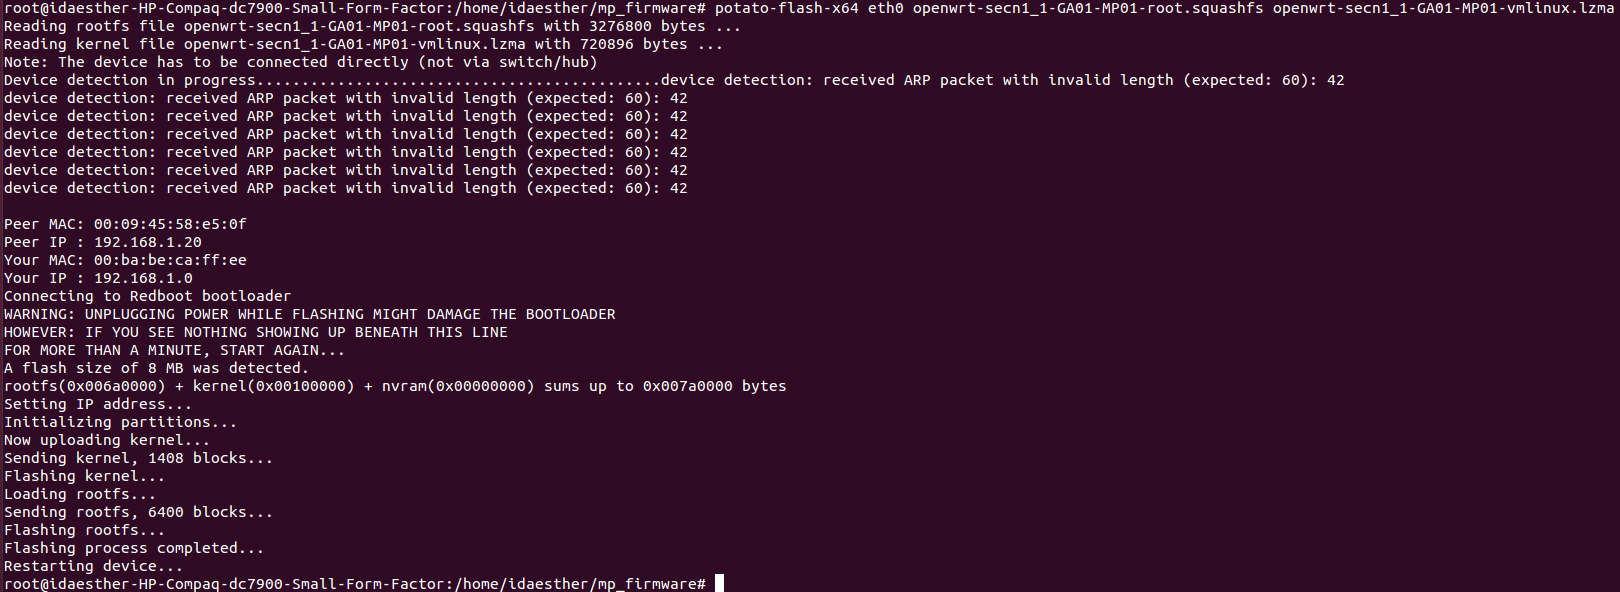
\includegraphics[width=1\textwidth]{potatoFlash.png}
  \caption [Flashing the Mesh Potato version 1]{\textbf{Flashing the Mesh Potato version 1.} This figure shows the flashing process from when we first flashed our Mesh Potato version 1}
  \label{fig:flashing}
\end{figure}


\subsubsection{Installing Firmware on Mesh Potato Version 2}
The process of upgrading the MP's firmware is simplified with the \gls{mp2}. With the \gls{mp1}, command shell (terminal) must be utilized in order install or upgrade the firmware. With the \gls{mp2}, firmware upgrade can be done from the \gls{secn} web interface (more information about the interface can be found in section \ref{subsec:interface}). Extra functionality has been added to the interface from \gls{mp1} to \gls{mp2}. Under "Advanced" in the interface an extra tab called "Firmware" is added. Under this tab the firmware upgrade can be executed. When the "Firmware"-button is pressed, a new windows pops up where you have to add the firmware file. The firmware for \gls{mp2} can be found here: \url{http://download.villagetelco.org/firmware/secn/unstable/mp02/SECN-2.0/SECN-2.0-RC4/}.

\subsection{The SECN Web Interface}
\label{subsec:interface}

\begin{figure}[t]
  \centering
      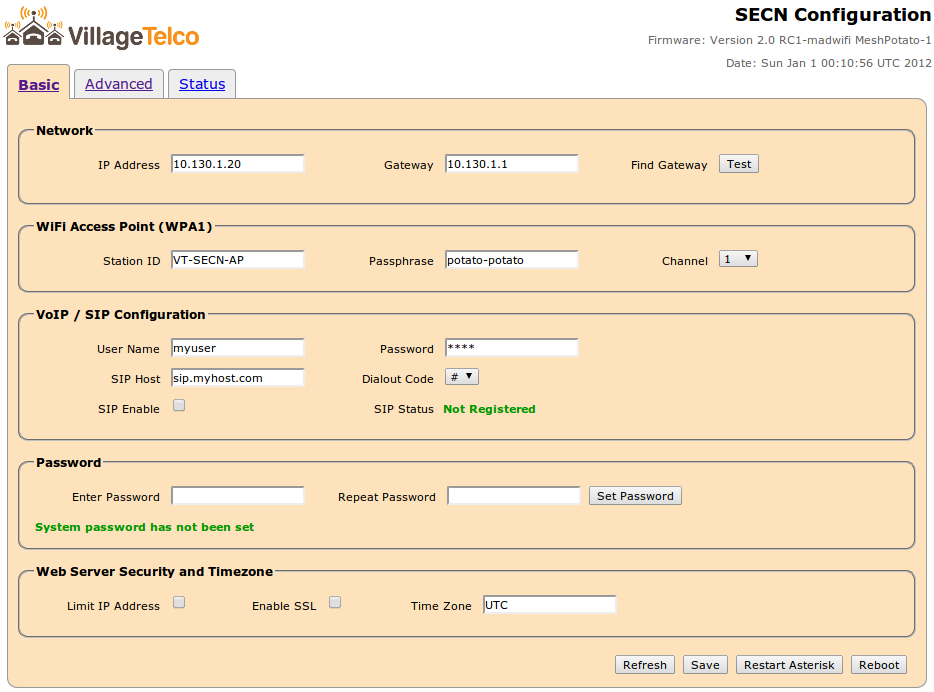
\includegraphics[width=1\textwidth]{webinterface.png}
  \caption [Web interface]{\textbf{Web interface.} Displays the MP's web interface.}
  \label{fig:webinterface}
\end{figure}

Village Telco provides a SECN web interface for configuration and management of individual \glspl{mp}. This web interface can be accessed by entering the \gls{ip} address of the \gls{mp} in a browser, as shown in \fref{fig:webinterface}. To be able to do this, the PC must be on the same subnet (exact same prefix) as the \gls{mp}.    

The web interface allows the user to alter different settings on the \gls{mp}. The user can, for example, change the \gls{ip} address of the device, set up the WiFi \gls{ap}, conduct \gls{voip}/\gls{sip} configurations, change/set password and configure web server security. The web interface also allows the user to alter more advanced settings. To get a detailed description of the web interface, see the SECN User Guides in Appendices \ref{chp:appendixB} and \ref{chp:appendixC}.



\section{QUICK Box}
The Mesh Potatoes and Village Telcos were created to get voice and data connection to areas where services like these are non-existent or too expensive for the average person. As of now, the \glspl{mp} have been set up to create networks of different size in villages all over the world. We want to expand this solution by looking at its mobility and its usage on the go. We want to make a box that has high adaptability, enabling it to easily be used in several different scenarios, under different conditions and by different people, all with different needs. The box must be user friendly, so there are no room for misunderstandings or mistakes. The box should be ready to go in any situation. QUICK stands for Quick User-friendly Internet-providing Communications Kit. 

\begin{itemize}
\item [] \textbf{Q}uick - The box should be easy to set-up, and include all manuals necessary to get started with the box, and to provide Internet access to the network. Scripting could be used in order to automate the set-up process. 
\item [] \textbf{U}ser-Friendly - The manuals should be easy to use, both by technical and "non-technical" people. 
\item [] \textbf{I}nternet-Providing - There should be manuals explaining how to connect the MP to various types of up-links. 
\item [] \textbf{C}ommunication - In today's society, and especially during emergency situations, it is crucial to have the possibility to communicate, both within a community, and with the outside world.
\item [] \textbf{K}it - Our solution will be delivered in a mobile suitcase. 
\end{itemize}

 
\subsection{Previous/Similar work}

\subsubsection{Go Box} Something similar has been done before by Keith Williamson, a volunteer in the Village Telco community. His idea of utilizing the Mesh Potatoes in emergency situations started with his interest in amateur radios, and the use of radios in emergency situations. He put together a "go box" by using a waterproof Pelican 1200 case. This case contained a bracket holding the Mesh Potato, a rechargeable Li-Ion or Li-Poly battery, telephone handset and a junction box to provide an on/off switch \cite{keith}. The \gls{quick} box differ in some ways from the "go box" made by Williamson. The main difference between the "go box" and the \gls{quick} box is the \gls{quick} box is based on the \gls{mp2}-basic, while the "go box" is created using \gls{mp1}. Since the \gls{quick} box is based on the \gls{mp2}-Basic, it is not possible to add a phone to our solution. Another difference is that the \gls{quick} box includes everything needed for an installation. The \gls{quick} box is therefore more comprehensive than the "go box".

\subsubsection{AfrikaBurn}
AfrikaBurn is a "Burning Man" festival in Tankwa Town in the Karoo (South Africa) that is held once a year \cite{whatisafrikaburn}. This is a festival with focus on art and freedom of expression. Instead of using money, the festival attendants are inspired to trade different types of goods with each other. A Village Telco has been established at this festival a few years now. Free-standing phone boots with Mesh Potatoes powered by solar panels has been set up at the festival area. The first year five phone boots were set up around the festival area. Since it were few numbers to call, the calling became sort of random. This gave a  "ChatRoulette" like effect, only with phones instead. The second year some aspects were improved from the previous year. The boots had production \glspl{mp}, no lighting and new sleeves. A netbook was brought with them, and this acted as a gateway \cite{africaburnforavillagetelco,africaburnsagainforavillagetelco}. 

\subsection{Key Components}
The key components of the \gls{quick} box is described in \tref{tab:components}. 

\begin{center}
\begin{table}[t]
\caption{\label{tab:components}The components of the QUICK box}
    \begin{tabular}{ | l | p{9cm} |}
    \hline
    \textbf{Component} & \textbf{Description and purpose} \\ 
    \hline
    Access point for Internet &  Mesh Potato version 2.\\ 
    \hline
    Suitcase/box &  A suitcase made of high quality plastic coated with aluminium foil. Strengthened edges and corners of aluminium and steel. It has a soft-padded interior. A solid handle for carrying. Dimensions: 455x330x152 (width, depth, height). Weight: 2,6 kg. \\ 
    \hline
    Power supply & A gel battery (12 V and 5 Ah). No need for maintenance. The battery acid is bound in a viscous gel. This prevents leakage, even when the battery is mounted horizontally. Long lifetime and safe to handle. The battery is fully closed, and do not need refill of battery water. No hydrogen gas or other gas might leak. When the battery is charging no gas or acid vapor is emitted, hence the battery can be placed in narrow or enclosed spaces. The battery withstands multiple discharges. The gel battery is ideal for seasonal or occasional use, since it have a slow self-discharge tempo, and a good ability to recover after deep discharging. Dimensions: 114x69x109. Weight: 2,16 kg. \\
    \hline
	Solar panel & Solar panel from Multicomp with item number: MC-SP10-GCS. Power rating: 10 W. Power Voltage Max: 17 V. Dimensions: 357x280x18.\\
	\hline
	Charge regulator & Regulator for 12 V solar panel. Protects the battery from overcharging and discharge. Capacity: 100 W / max. 7 A. Overcharging protection: 14.5 V. Discharge protection: <10,5 V. Three diodes shows charging, high voltage and low battery voltage. \\
	\hline
	Manuals & Different manuals for providing Internet access to the MP, and a manual explaining how to get started with the QUICK box.\\
	\hline
	CD with Linux Ubuntu & A CD with Linux Ubuntu is provided.\\
	\hline
	USB-stick & The USB-stick contains a script that can be run in order to provide Internet access to the MP via a PC.\\
	\hline
	Necessary cables & An Ethernet cable is provided in order to connect the MP to a PC, and an extra power cord is added in case there is a power outlet available. \\
	\hline
    \end{tabular}
   \end{table}
\end{center}

\clearpage

\subsection{Creating the QUICK Box}
This section describes how we created the \gls{quick} box from scratch. The box is delivered with a Mesh Potato that is pre-configured with an unique \gls{ip} address. The suitcase contains a CD with Linux Ubuntu in case the user does not already have it installed. It is necessary to have Linux in order to execute all the configurations and set-ups provided in the box. The case also contains necessary cables and detailed descriptions on how to connect to the different up-links, in order to provide Internet access to the network. \fref{fig:boxinmaking} shows the box in the making.


\begin{figure}[b]
  \centering
      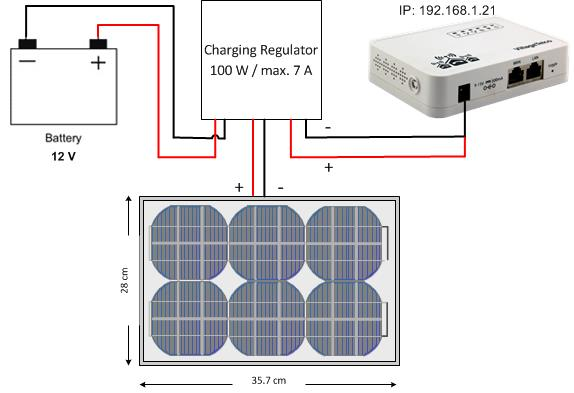
\includegraphics[width=0.9\textwidth]{emergencybox.jpg}
  \caption [The composition of the \gls{quick} box]{\textbf{The composition of the \gls{quick} box.} This figure shows how the key components in the \gls{quick} box is conjoined together.}
  \label{fig:emergencybox}
\end{figure}

\paragraph{Conjoining the components of the QUICK box.}
The key components that we used to construct the box was a charge regulator, a gel battery, a solar panel and an \gls{mp2}. These components were conjoined as shown in \fref{fig:emergencybox}. The charge regulator is connected to all the components, and is used in order to not overcharge the battery. The charge regulator was initially built for another type of solar panel than the one we chose to use. This means that the concomitant plugs could not be used. These plugs were cut of and we soldered on new wires.  

New wires were soldered on the charge regulator, one was connected to the MP's power cord, while the other two was connected to the battery and to the solar panel. Before connecting everything together we used a multimeter to measure the voltage of the solar panel. We placed the solar panel under a bright light (lamp) to see if it had any impact, which it did. We used the multimeter to check the battery as well, which was fully charged, with a voltage of a little over 13 V. 
We first connected the solar panel, then the battery, and at last the Mesh Potato. When everything was conjoined correctly, the \gls{mp} turned on. \fref{fig:ferdigbox} shows our final prototype of the \gls{quick} box. 

\begin{figure}
        \centering
        \begin{subfigure}[t]{0.4\textwidth}
                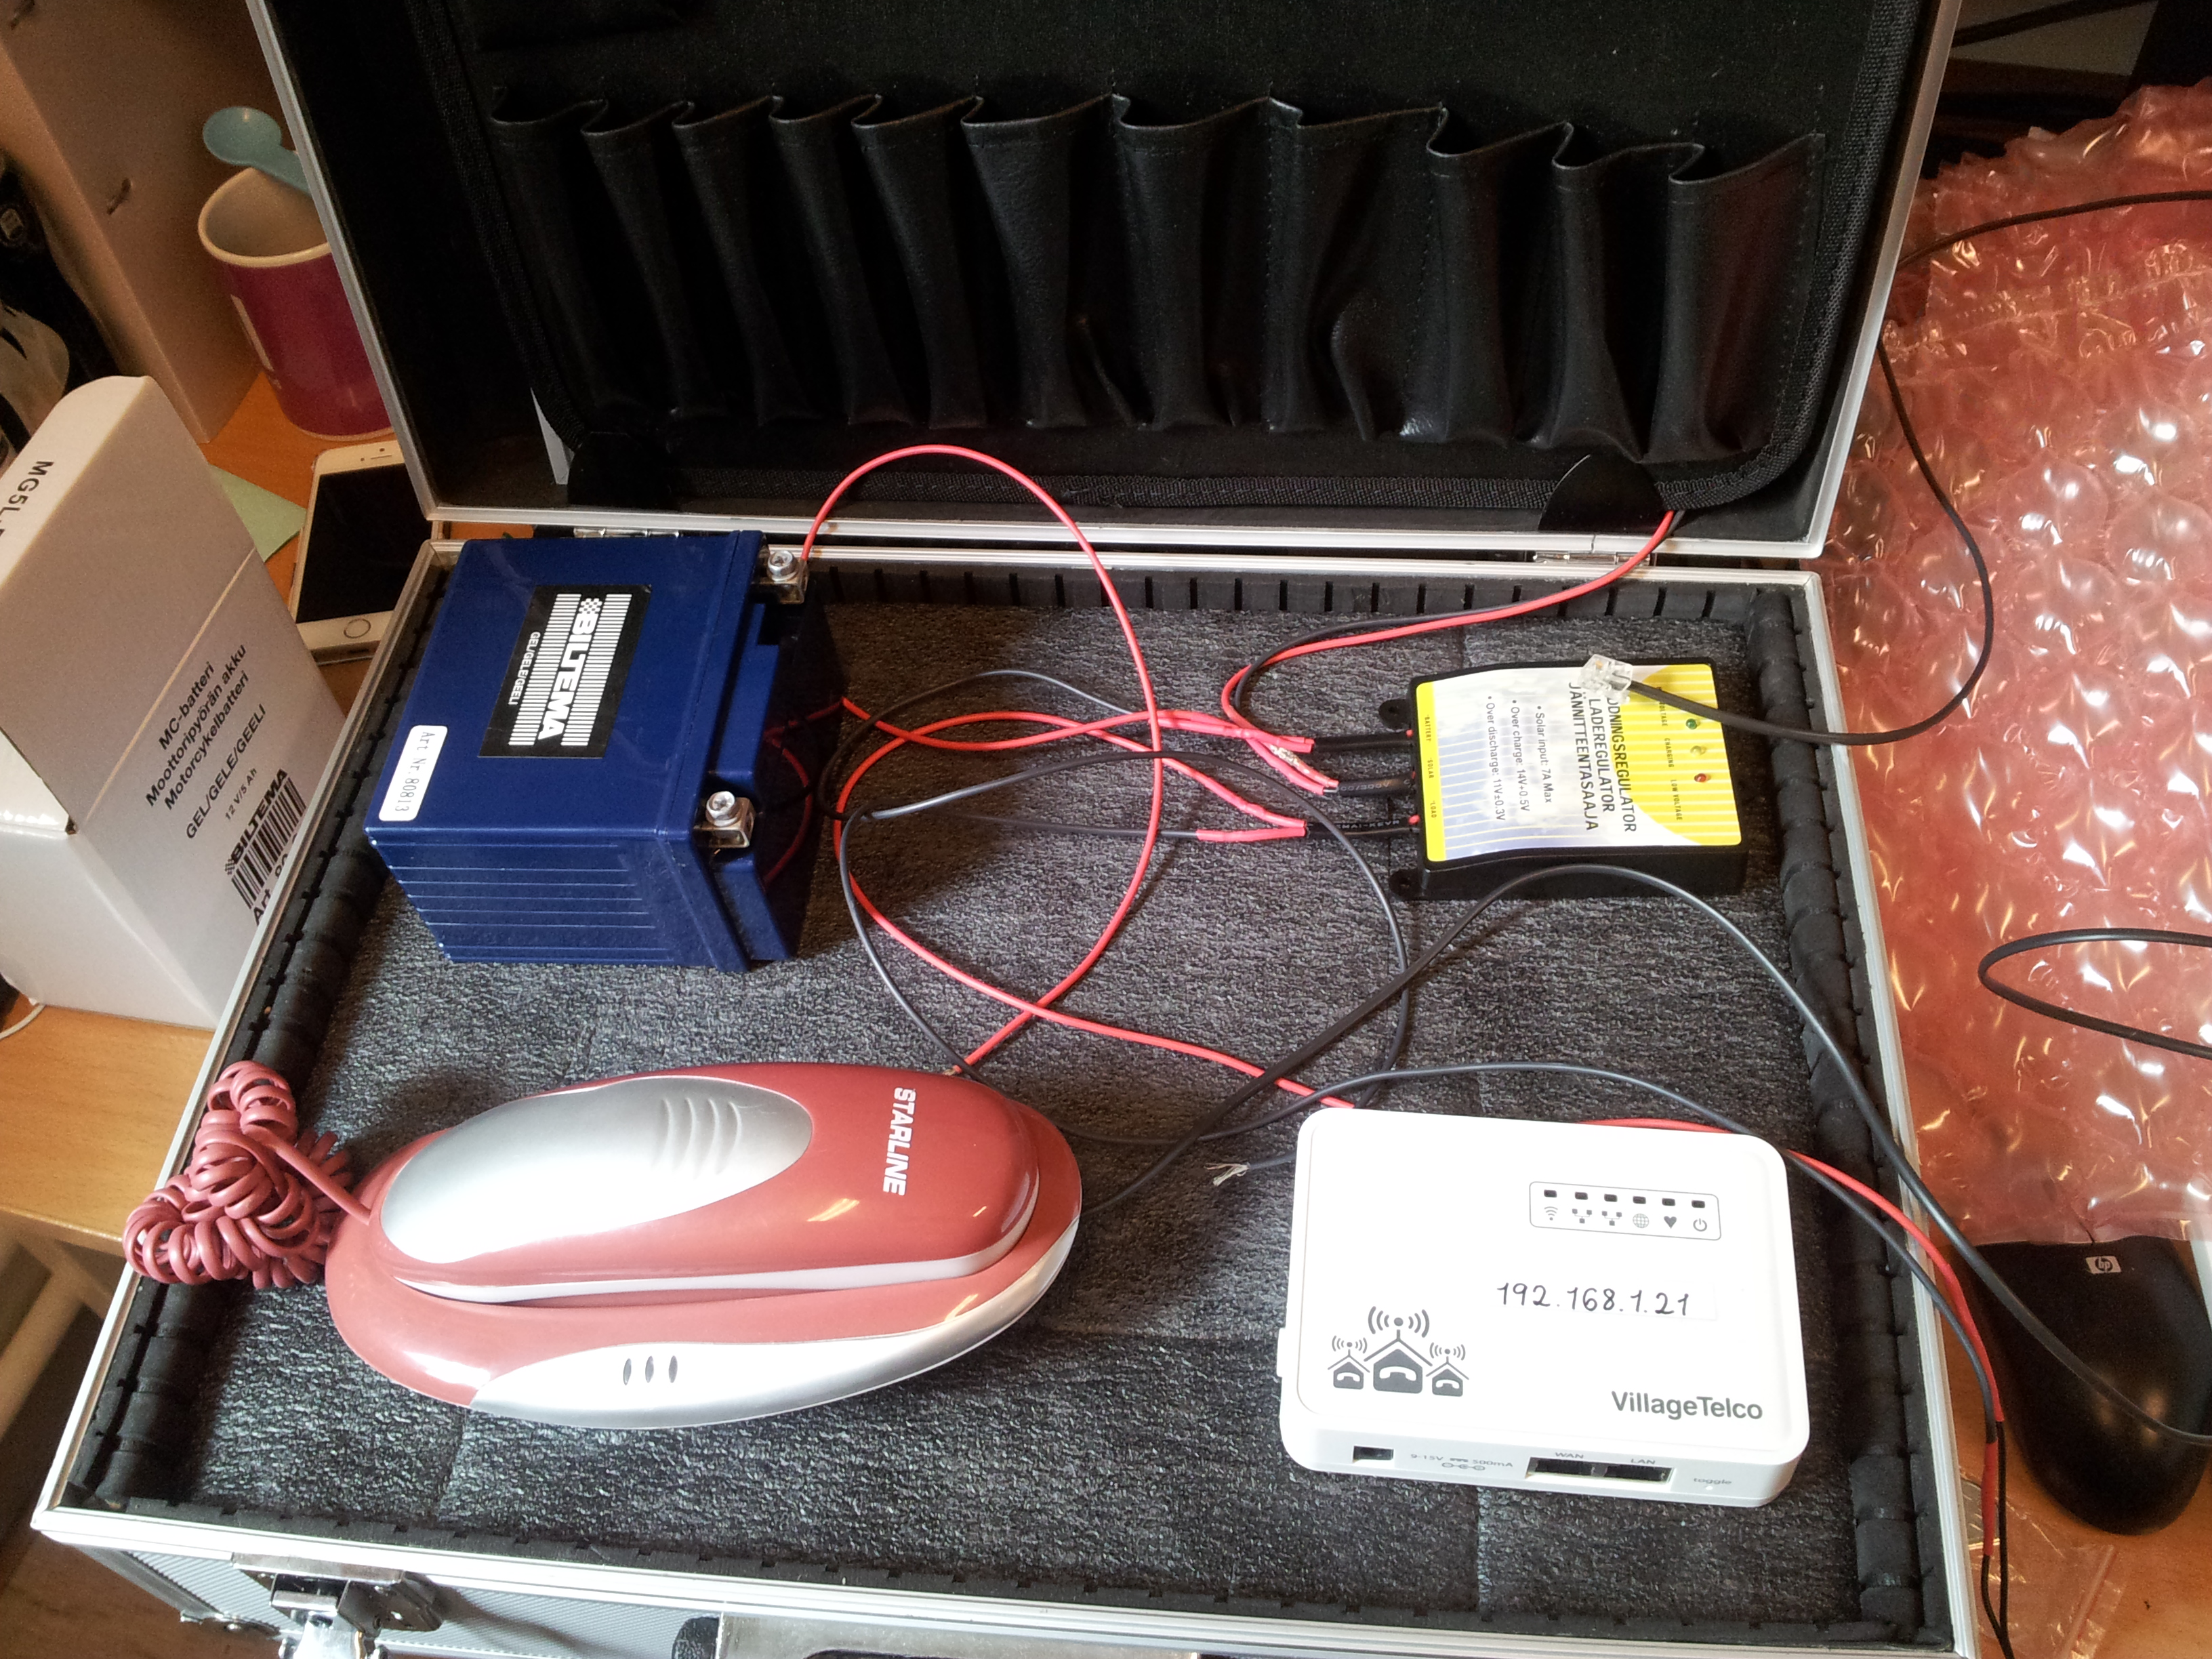
\includegraphics[width=\textwidth]{boxinmaking2}
                \label{fig:boxinmaking2}
        \end{subfigure}
        \begin{subfigure}[t]{0.4\textwidth}
                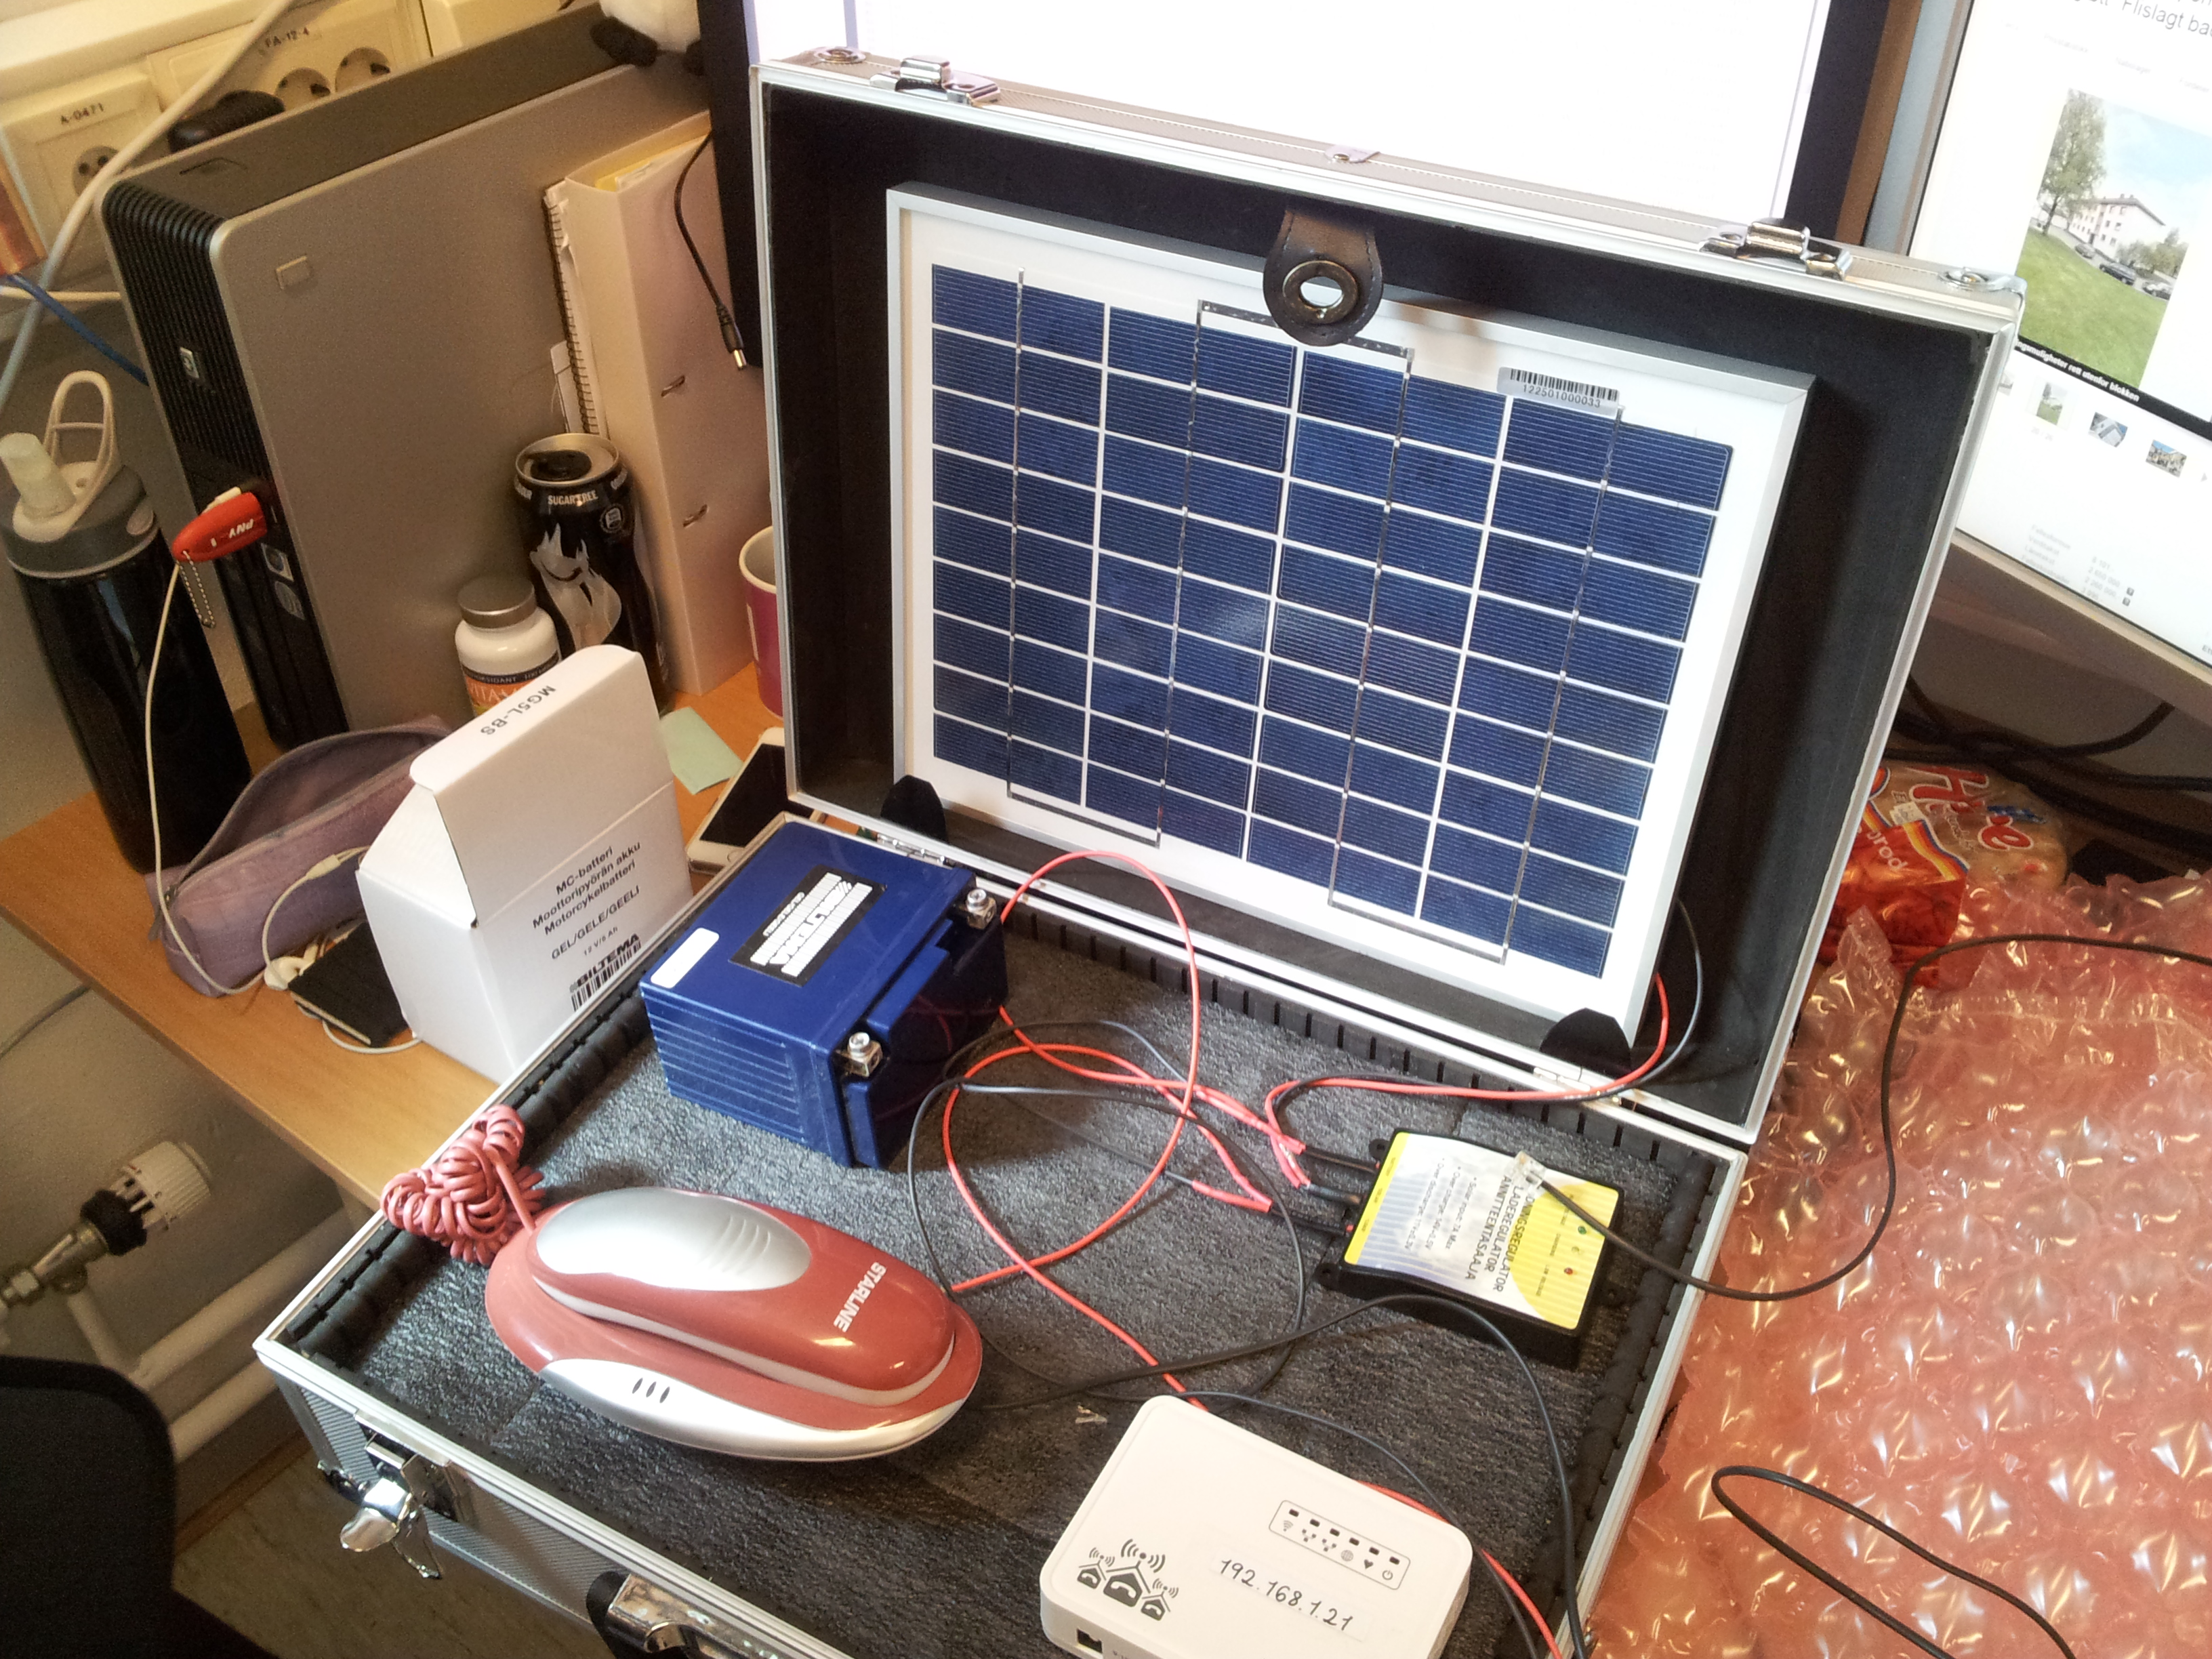
\includegraphics[width=\textwidth]{boxinmaking4}
                \label{fig:boxinmaking}
        \end{subfigure}
         \begin{subfigure}[t]{0.3\textwidth}
                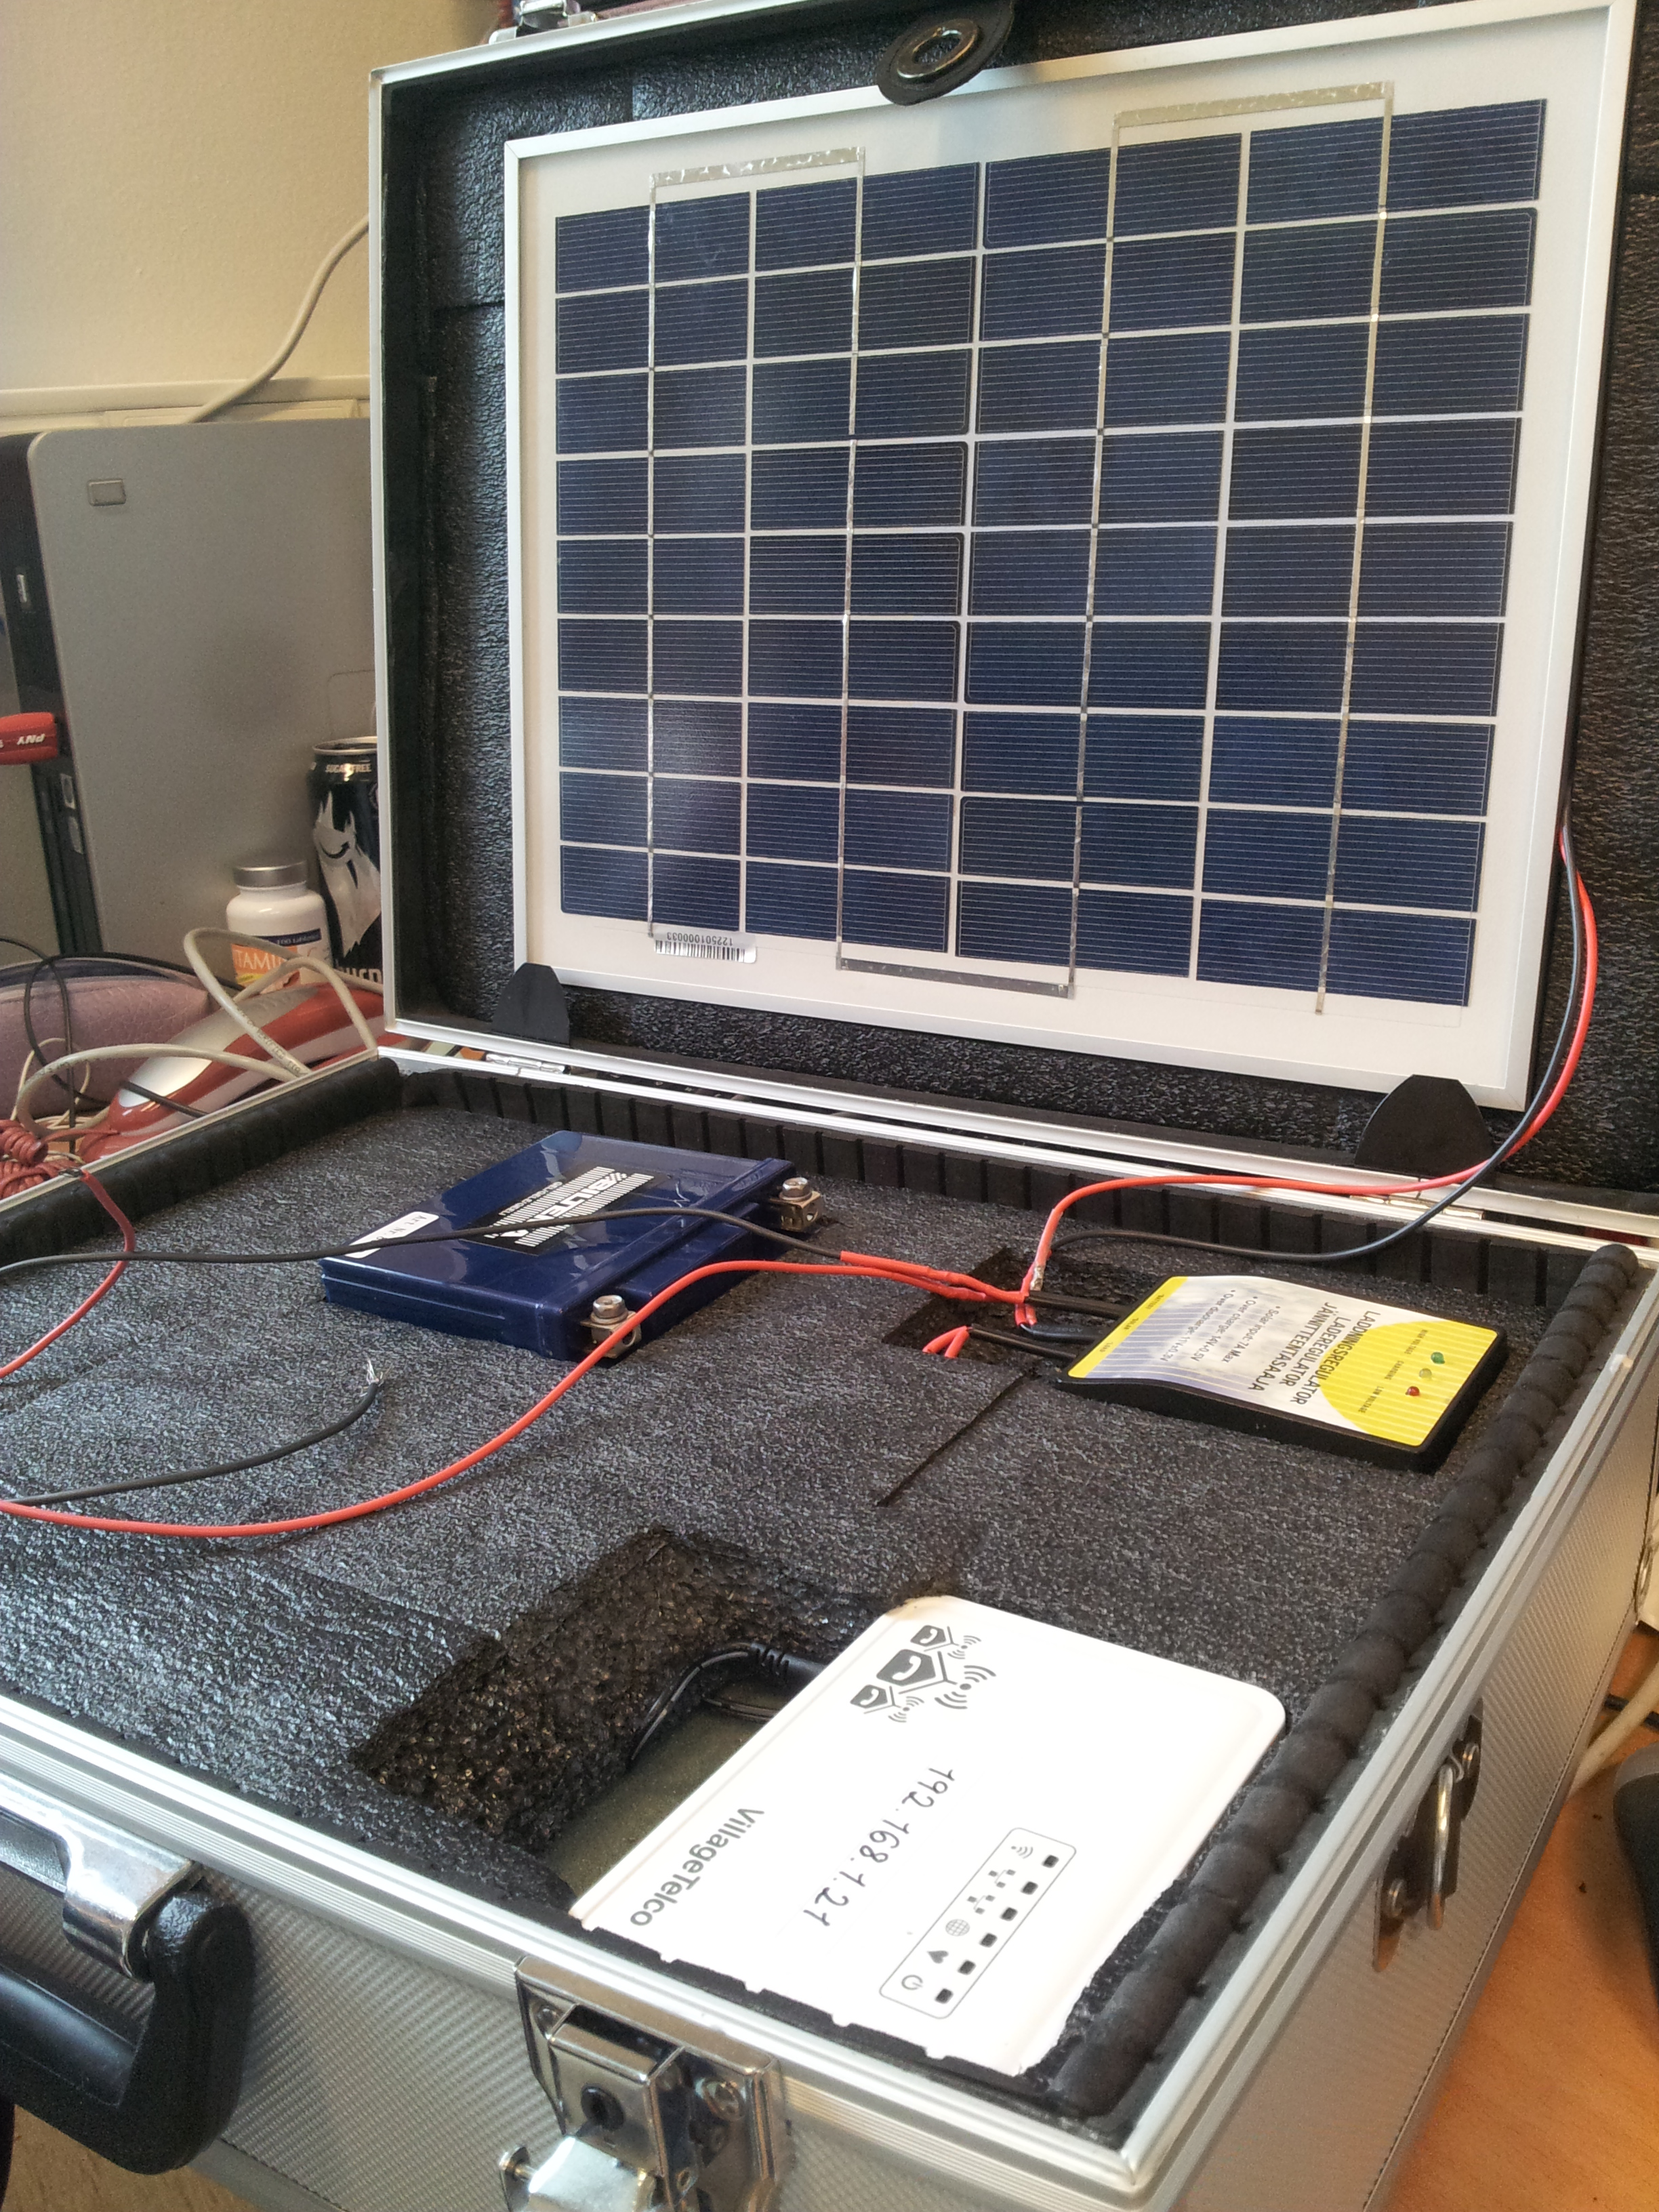
\includegraphics[width=\textwidth]{boxinmaking3} 
                \label{fig:boxinmaking3}
        \end{subfigure}
        \begin{subfigure}[t]{0.4\textwidth}
                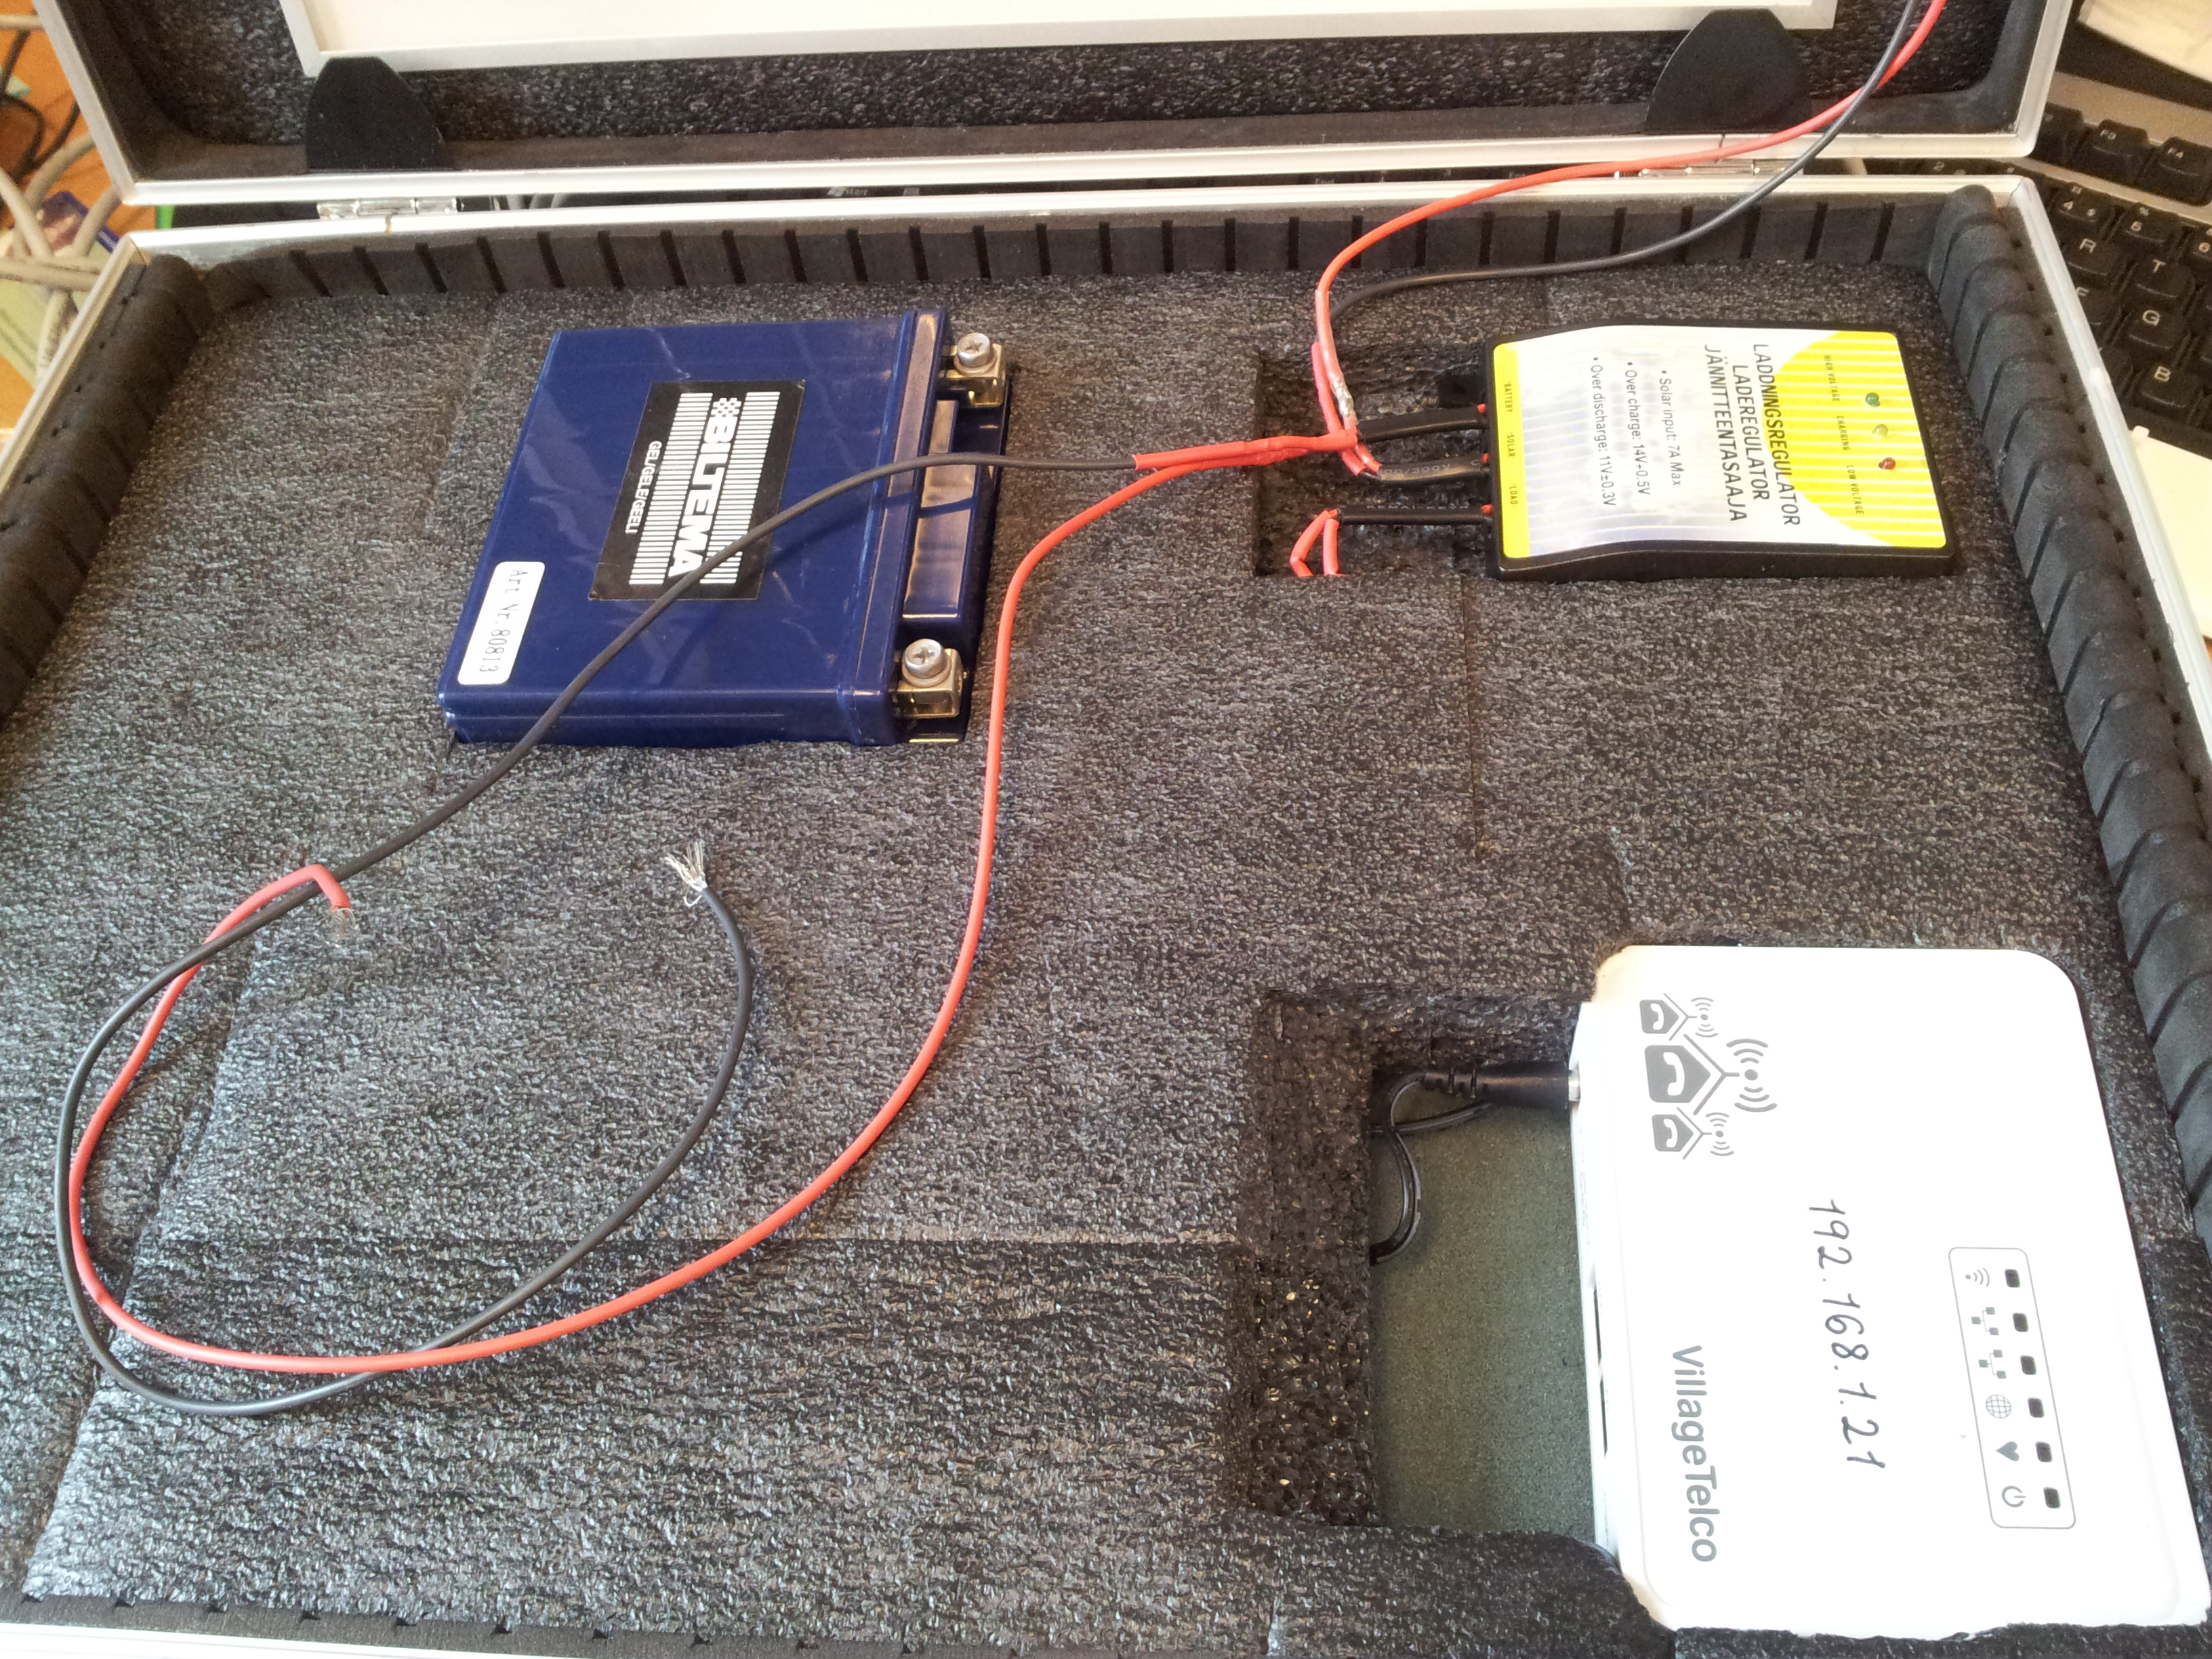
\includegraphics[width=\textwidth]{boxinmaking} 
                \label{fig:boxinmaking4}
        \end{subfigure}
\caption{Building the QUICK box.} \label{fig:boxinmaking}
\end{figure}

\begin{figure}
        \centering
        \begin{subfigure}[t]{0.4\textwidth}
                \includegraphics[width=\textwidth]{ferdigbox1}
                \label{fig:ferdigbox1}
        \end{subfigure}
        \begin{subfigure}[t]{0.4\textwidth}
                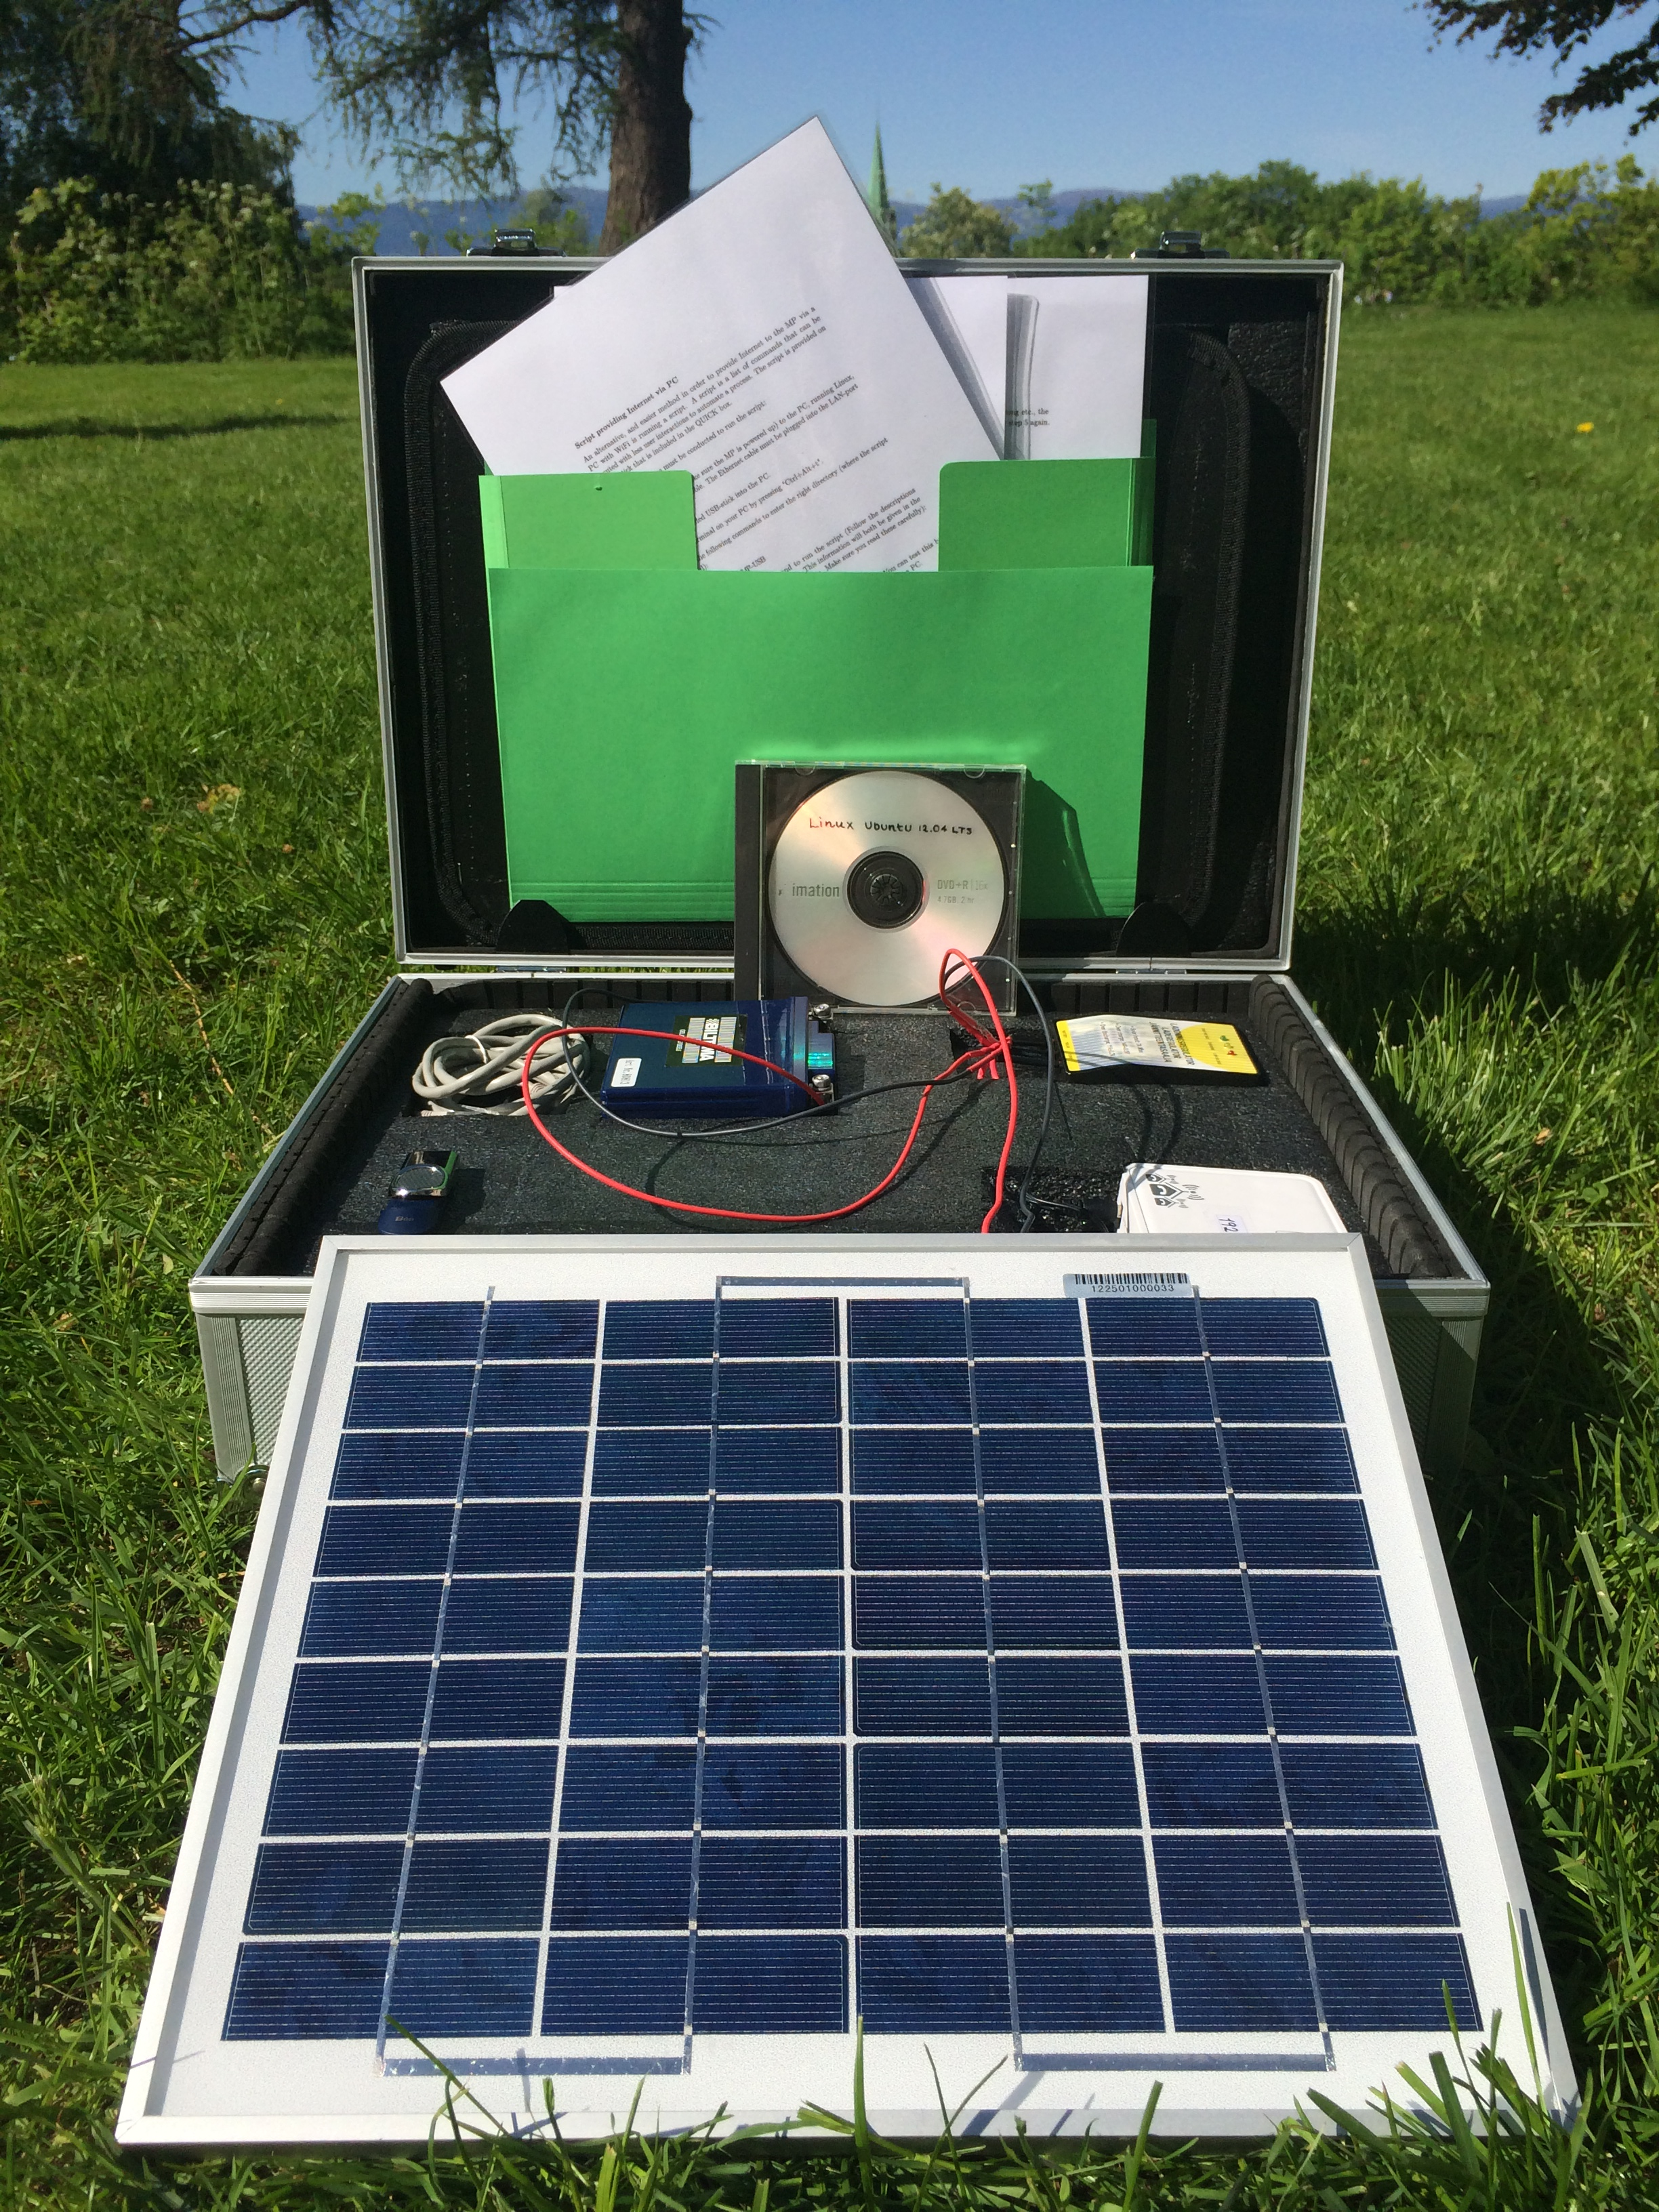
\includegraphics[width=\textwidth]{ferdigbox2}
                \label{fig:ferdigbox2}
        \end{subfigure}
         \begin{subfigure}[t]{0.81\textwidth}
                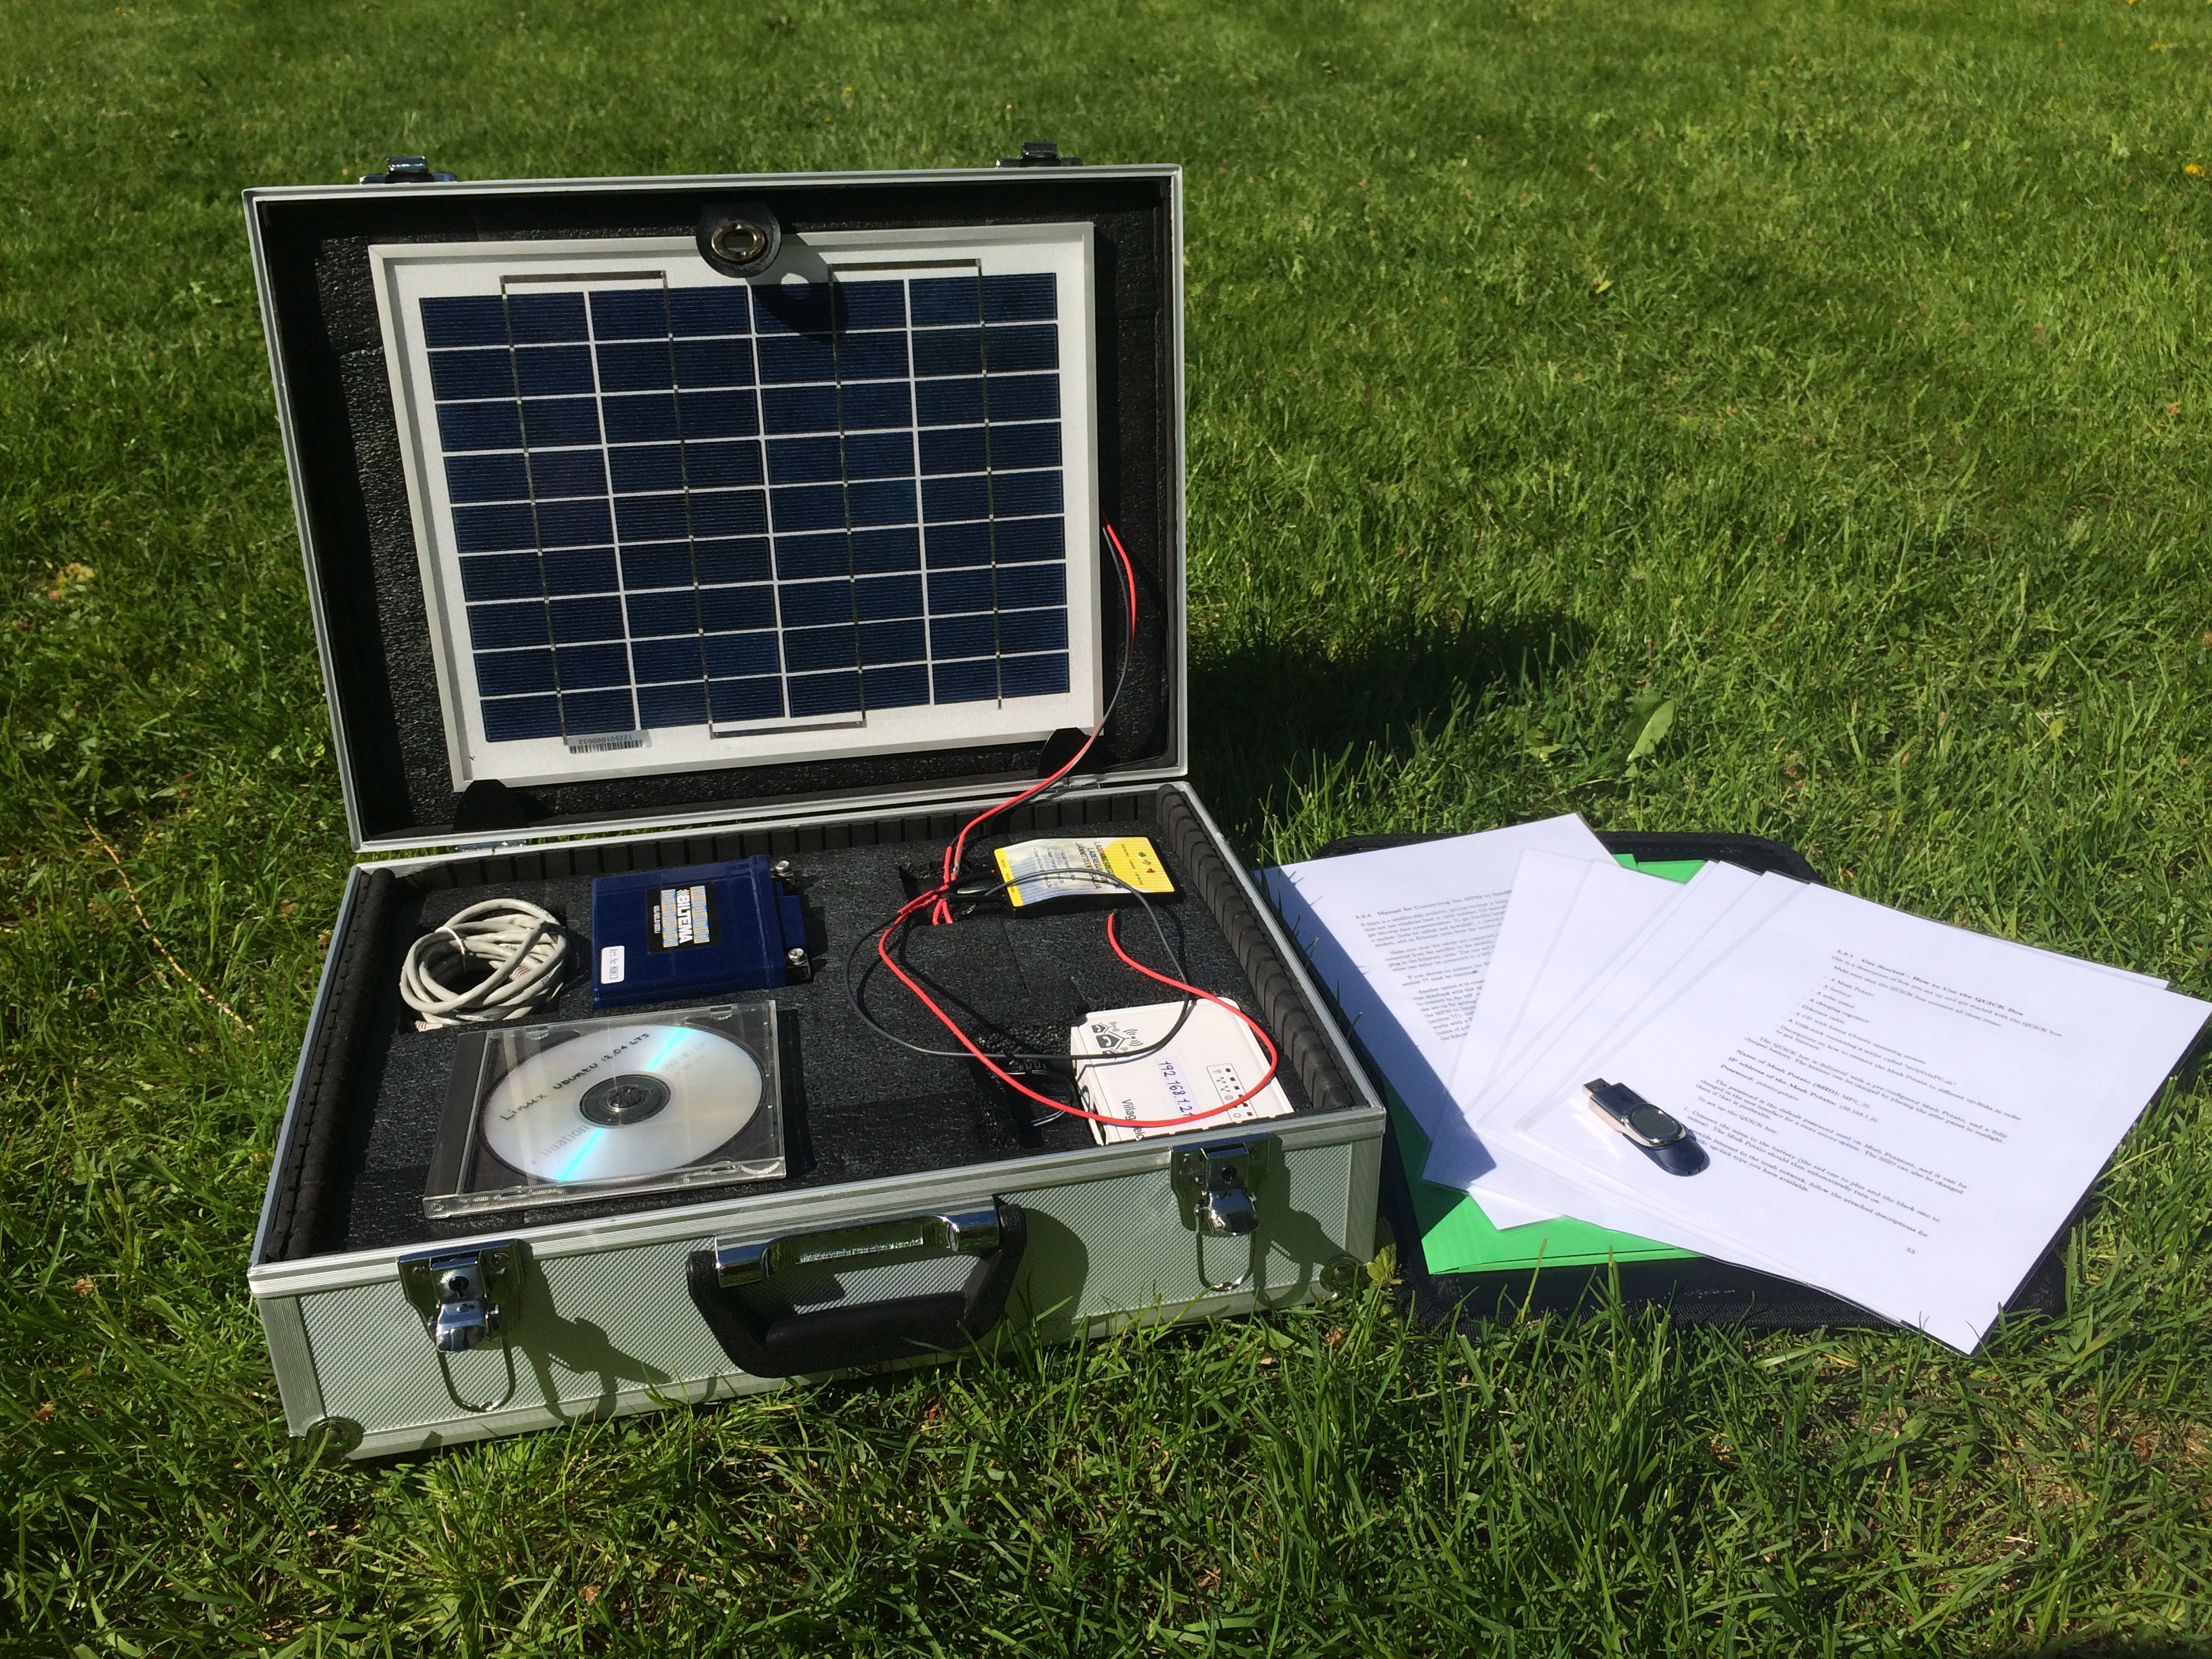
\includegraphics[width=\textwidth]{ferdigbox3} 
                \label{fig:ferdigbox3}
        \end{subfigure}
\caption[Final prototype of the QUICK box]{\textbf{Final prototype of the QUICK box.} This figure shows the final prototype of the QUICK box including everything necessary for a quick roll-out. As shown, there is room for adding a telephone inside the box. This can be included with the \gls{mp2}-Phone.} \label{fig:ferdigbox}
\end{figure}


\paragraph{Configuring and upgrading the QUICK Box.}
When the \gls{quick} box is delivered, the Mesh Potato is already set-up and configured with an unique \gls{ip} address, and running the latest version of the \gls{secn} firmware. The processes of upgrading and configuring the MP are described in sections \ref{subsec:configuring} and \ref{subsec:upgrading}. These descriptions are attached in the QUICK box.

\clearpage

\subsection{Battery and Charging Calculations}
All the calculations done in this section is based on the components described in \tref{tab:components}. 

\subsubsection{Charging with solar panel}
How long it will take for the solar panel to charge the battery from a fully discharged state to a fully charged state, depends on how much sun there is. The following calculations are based on the peak value of the solar panel (10W). 

The solar panel capacity is:
$$Amp = \frac{Watt}{Volt} = \frac{10 W}{17 V} = 0.59 Ampere$$

When charging batteries it is important to take the charging factor into consideration. This factor is the ratio between supplied capacity and submitted capacity. The charging factor varies depending on battery type. For the gel battery used in the \gls{quick} box the factor is roughly 1.2. The charging factor does not have an annotation. 
If the battery is completely discharged it will take: 

$$Amp\times Hours = AmpHours \Rightarrow Hours =\frac{AmpHours}{Amp} = \frac{5 Ah\times 1.2}{0.59 A} = 10.17 Hours$$

to fully charge it. 

This calculation does not take into consideration that the solar panel might have to charge the battery while the \gls{mp} is running. The effect from the solar panel to the battery will then decrease. 

\subsubsection{Charge while MP01 is running}
The capacity from the solar panel with the MP01 running is: 
$$Amp = \frac{Watt}{Volt} = \frac{10-2.5 W}{17 V} = 0.44 Ampere$$

The time it will take to fully charge the battery from fully discharged condition will then be: 
$$Amp\times Hours = AmpHours \Rightarrow Hours =\frac{AmpHours}{Amp} = \frac{5 Ah\times 1.2}{0.44A} = 13.6 Hours$$

\subsubsection{Charge while MP02 is running}
The capacity from the solar panel with the MP02 running is: 
$$Amp = \frac{Watt}{Volt} = \frac{10-0.75 W}{17 V} = 0.54 Ampere$$

The time it will take to fully charge the battery from fully discharged condition will then be: 
$$Amp\times Hours = AmpHours \Rightarrow Hours =\frac{AmpHours}{Amp} = \frac{5 Ah\times 1.2}{0.54A} = 11.1 Hours$$

In South Africa in December, for example, the number of sun hours per day is approximately 14. In June the number of sun hours is approximately 10.5. These numbers are best case, since cloudy weather has not been taken into consideration. This means that it is possible to fully charge the battery in the course of a day, but this may not always be the case. The following calculations show how long the battery can provide the Mesh Potato with power when fully charged, without the solar panel charging the battery simultaneously. 

\subsubsection{With fully charged battery - MP01}
This calculation takes into account that the solar panel is disconnected from the battery. With the components described in \tref{tab:components} the number of hours the \gls{mp1} can last with a fully charged battery is: 

$$Amp = \frac{Watt}{Volt} = \frac{2.5 W}{12 V} = 0.208 Ampere$$
$$Amp\times Hours = AmpHours \Rightarrow Hours = \frac{AmpHours}{Amp} = \frac{5 Ah}{0.208 A} = 24 Hours$$

\subsubsection{With fully charged battery - MP02}
This calculation takes into account that the solar panel is disconnected from the battery. With the components described in \tref{tab:components} the number of hours the \gls{mp2} can last with a fully charged battery is: 

$$Amp = \frac{Watt}{Volt} = \frac{0.75 W}{12 V} = 0.06 Ampere$$
$$Amp\times Hours = AmpHours \Rightarrow Hours = \frac{AmpHours}{Amp} = \frac{5 Ah}{0.06 A} = 83 Hours$$

As the calculations show, the MP02 use much less power and can therefore last on the battery almost four times longer than the MP01. 


\subsection{Possible Improvements}
As mentioned, the \gls {quick} box is fairly easy and simple, and leaves room for improvements. There should be an on/off switch in order to spare battery capacity. This on/off switch would be placed between the battery and the regulator. Unless a measuring instrument is available to check the voltage, there are no way for the user to know the remaining battery capacity. This might be very useful in situations where communication is vital and the hours of battery lifetime and sun hours are limited. 

The battery used is a gel battery. They are less explosive than the lithium batteries, and are better suited to be placed into enclosed spaces that may get hot. The downside of the gel batteries is their weight, since they are very heavy. Our aim is to make a case that is portable, a lighter battery would be preferable. Under the requirement of being portable a factor to keep in mind is that it is not allowed to bring lithium batteries on airplanes. This means that if we chose to use a lithium battery in our solution, a regular person would not be allowed to bring the \gls{quick} box on an airplane. When it comes to relief organizations, this might not be a problem since they transport equipment in their own airplanes, for example Hercules. 

The \gls{mp2} is small (much smaller than the \gls{mp1}), and a powerful solar panel does not take much space, so there is no need for a suitcase of the size we have used. A smaller case, that is lighter and easier to handle, would make the solution even more portable. 

Our main focus was to make something that worked and that was safe. We did not focus on aesthetics and appearance. This is therefore also an area with room for improvements. 

 
\section{Different Scenarios Where a Quick Roll-out Might be Necessary}
Everyday there occur situations in the world that might affect the modern communications system, or causes a need for one. These situations can range from big natural disasters, like the tsunami in Japan, to temporary refugee camps. Also more festive situations, like a music festival, can utilize a quick roll-out communications system. The following sections describes some of the scenarios where the \gls{quick} box might be useful. 

\subsection{Natural Disasters}
A natural disaster is defined as: \textit{any event or force of nature that has catastrophic consequences, such as avalanche, earthquake, flood, forest fire, hurricane, lightning, tornado, tsunami, and volcanic eruption} \cite{naturalDisaster}.

All over the world relief organizations are ready to help if an unexpected situation occurs. These groups of people have the equipment, knowledge, experience and funding to help people in desperate need. Where are their help needed? Or if they hear about the disaster and the first respond team is in place, how do they report back about the situation? How do they communicate with each other to work more effectively and help the ones in desperate need? There is no doubt that there is a need for a simple, fast, and reliable communications system.

When a natural disaster strikes, it is hard to know the extent of it, which  again makes it difficult to predict how the communications systems would be affected. This unpredictability makes it important to always have a back-up plan to the back-up plan. History shows that cell phone service is not a reliable service during an emergency situation. During 9/11 the system became heavily overloaded, and when hurricane Katrina hit, 70\% of the cell phone towers were knocked down. People might think that if they live in a big metropolitan they will be safe, but this is not necessarily the case \cite{disasterComm}. In addition, these examples are from the western world. The western communications systems tend to be more robust initially, compared to the ones in developing countries. 

When looking at the developing world, which unfortunately is often more exposed to natural disasters, the situation is different. According to \cite{DevelopingWorld, 360} developing countries are in an larger extent affected by natural disasters than the developed world. The reason for this can be explained by the economic status of the country, both in how the country is prepared for a disaster and in how fast they can rebuild and recuperate after a natural disaster. Developing countries often lack the infrastructure needed to quickly and efficiently provide aids to the ones affected. According to Baxter \cite{360}, a natural disaster could set back a developing country many years in development.  

People are extremely dependent on having the ability to communicate when natural disasters occur. It is crucial to have the possibility to inform others about the current situation and about what is needed at the disaster area. Time can be the difference between life and death in situations like these. Employing \gls{quick} boxes could be a good solution in situations like these. 

In the next sections, two examples of recent natural disasters, respectively from a developed country, and an underdeveloped country. The examples shows how the situation was handled, and if there were emergency communications systems available. 

\subsubsection{Hurrican Sandy}
Hurricane Sandy hit big parts of the Caribbean, as well as the south-east parts of the Unites States at the end of October 2012 \cite{WikiSandy}. As many as 25\% of the citizens in the affected areas lost cell phone coverage, and even more lost electricity. Communication is a challenge both during and after a natural disaster. It may also be difficult for first responders (like fire fighters, police, etc.) to communicate. No single communication system is fault free, and it is therefore smart to have a back-up communications system. Satellite communications was used, but the phones are expensive and the lines can be oversaturated if others are trying to connect to the network simultaneously. A small aperture terminal (VSAT) trailer was used to act like a satellite ground station. Finding a good spot for the trailer can be tricky, it requires clear view to the sky and it can not be placed too close to a tall building. The Red Cross launched an emergency preparedness application for smart phones. The application had a peak in downloads right before the hurricane hit, but when the commercial wireless network failed, they had to go back to the old way of spreading information; distributing paper files, going from house-to-house to check up on people, give information word-by-mouth and using bullhorns \cite{hurricaneSandy}.

\subsubsection{Philippines}
November 8 2013 the typhoon Haiyan, a powerful tropical cyclone, struck and destroyed parts of south-east Asia, in particular the Philippines. Haiyan is the strongest hurricane in wind speed ever recorded. The hurricane had the highest number for casualties, killing over 6,268 people in the Philippines alone \cite{wikiHaiyan}. International humanitarians and the Philippine government were warned about the storm in advance, but nobody could anticipate its viciousness. Some of the first teams on the spot was communication experts. Their assignment was to help with coordination, and make sure information was spread as desired \cite{disasterResponse}.

Numerous of relief organizations contributed with their help after the typhoon struck. They helped with everything from food and shelter, to collecting donations. The United Nations World Relief Programme were among the helpers, and they helped setting up emergency communications systems \cite{philippines}. In addition to this, amateur radio operators helped with communication both during and after the disaster. Due to power outages, the existing communications systems were down and there were no cell phone signals. By using radio, they could help keep track of the storm, and give important information (about evacuations and flooding). The radio was also used to help people communicate with their loved ones \cite{philippinesradio}. 


\subsection{Temporary Refugee and IDP camps}
We got a better understanding of refugee and IDP camps after conducting interviews with different relief organizations (for interview with respectively the Norwegian Refugee Council and CARE, see section \ref{sec:interviewnrc} and section \ref{sec:interviewcare}). 
Not all refugee and IDP camps are as well established, like the one in Dadaab. Many camps are short-term, and are therefore in more need of a temporary communications system. In this case, setting up \gls{quick} boxes in the camp to provide the refugees/IDPs with Internet access could be an option. 

\subsection{Festivals}
Imagine you are at a music festival with your friends in a foreign country. There are thousands of people, and much activity. In a scenario like this, there are many reasons why an Internet connection would be beneficial. You could loose your friends, have to inform your friends about something urgent, inform the staff if an emergency situation occur and so on. Since it is very expensive to send text messages, make phone calls or use cellular networks abroad, it could be an idea to use the Mesh Potatoes to provide the people at the festival with Internet access. This could be set up by the organizers in advance. Although this adds an extra cost to the organizers, the people attending the festival can save a lot of money by refraining from using the expensive services available on their smart phones. The organizers could add an extra fee to prize of the festival pass, and it would probably still be beneficial for the people at the festival. 

\subsection{Breakdown of Mobile Towers}

The 10th of June 2011 Telenor had problems with one of their servers in Oslo. This problem caused a down time of 18 hours and affected 3 000 000 Telenor users \cite{listeNedetid}. Not only was this the biggest problem Telenor have had since they opened their mobile network in 1993, but it was also the longest downtime and had the highest number of affected users recorded in Norway. In addition to this it all happened in a period with severe flooding in big parts of eastern Norway, and made it difficult to reach emergency numbers. The fact that the problems occurred during the flooding made the situation much worse \cite{TelenorNede}.
